\documentclass[]{article}
\usepackage{lmodern}
\usepackage{amssymb,amsmath}
\usepackage{ifxetex,ifluatex}
\usepackage{fixltx2e} % provides \textsubscript
\ifnum 0\ifxetex 1\fi\ifluatex 1\fi=0 % if pdftex
  \usepackage[T1]{fontenc}
  \usepackage[utf8]{inputenc}
\else % if luatex or xelatex
  \ifxetex
    \usepackage{mathspec}
  \else
    \usepackage{fontspec}
  \fi
  \defaultfontfeatures{Ligatures=TeX,Scale=MatchLowercase}
\fi
% use upquote if available, for straight quotes in verbatim environments
\IfFileExists{upquote.sty}{\usepackage{upquote}}{}
% use microtype if available
\IfFileExists{microtype.sty}{%
\usepackage{microtype}
\UseMicrotypeSet[protrusion]{basicmath} % disable protrusion for tt fonts
}{}
\usepackage[margin=1in]{geometry}
\usepackage{hyperref}
\hypersetup{unicode=true,
            pdftitle={MAthesis},
            pdfauthor={Julia Joos},
            pdfborder={0 0 0},
            breaklinks=true}
\urlstyle{same}  % don't use monospace font for urls
\usepackage{natbib}
\bibliographystyle{plainnat}
\usepackage{longtable,booktabs}
\usepackage{graphicx,grffile}
\makeatletter
\def\maxwidth{\ifdim\Gin@nat@width>\linewidth\linewidth\else\Gin@nat@width\fi}
\def\maxheight{\ifdim\Gin@nat@height>\textheight\textheight\else\Gin@nat@height\fi}
\makeatother
% Scale images if necessary, so that they will not overflow the page
% margins by default, and it is still possible to overwrite the defaults
% using explicit options in \includegraphics[width, height, ...]{}
\setkeys{Gin}{width=\maxwidth,height=\maxheight,keepaspectratio}
\IfFileExists{parskip.sty}{%
\usepackage{parskip}
}{% else
\setlength{\parindent}{0pt}
\setlength{\parskip}{6pt plus 2pt minus 1pt}
}
\setlength{\emergencystretch}{3em}  % prevent overfull lines
\providecommand{\tightlist}{%
  \setlength{\itemsep}{0pt}\setlength{\parskip}{0pt}}
\setcounter{secnumdepth}{5}
% Redefines (sub)paragraphs to behave more like sections
\ifx\paragraph\undefined\else
\let\oldparagraph\paragraph
\renewcommand{\paragraph}[1]{\oldparagraph{#1}\mbox{}}
\fi
\ifx\subparagraph\undefined\else
\let\oldsubparagraph\subparagraph
\renewcommand{\subparagraph}[1]{\oldsubparagraph{#1}\mbox{}}
\fi

%%% Use protect on footnotes to avoid problems with footnotes in titles
\let\rmarkdownfootnote\footnote%
\def\footnote{\protect\rmarkdownfootnote}

%%% Change title format to be more compact
\usepackage{titling}

% Create subtitle command for use in maketitle
\newcommand{\subtitle}[1]{
  \posttitle{
    \begin{center}\large#1\end{center}
    }
}

\setlength{\droptitle}{-2em}
  \title{MAthesis}
  \pretitle{\vspace{\droptitle}\centering\huge}
  \posttitle{\par}
  \author{Julia Joos}
  \preauthor{\centering\large\emph}
  \postauthor{\par}
  \predate{\centering\large\emph}
  \postdate{\par}
  \date{14 August 2017}

\usepackage{setspace}
\doublespacing

\begin{document}
\maketitle

\begin{longtable}[]{@{}llrrrr@{}}
\caption{Time bins with age range, epoch name, mean age and
corresponding sample sizes (on individual, species and genus
level)}\tabularnewline
\toprule
bin & EpochBins & MeanBins & nIndividuals & nSpecies &
nGenera\tabularnewline
\midrule
\endfirsthead
\toprule
bin & EpochBins & MeanBins & nIndividuals & nSpecies &
nGenera\tabularnewline
\midrule
\endhead
(0,1e-06{]} & Modern & 0.0000005 & 240 & 58 & 17\tabularnewline
(1e-06,0.0117{]} & Holocene & 0.0058500 & 12 & 6 & 4\tabularnewline
(0.0117,0.126{]} & Upper Pleistocene & 0.0688500 & 46 & 15 &
7\tabularnewline
(0.126,0.781{]} & Middle Pleistocene & 0.4535000 & 46 & 9 &
6\tabularnewline
(0.781,2.59{]} & Lower Pleistocene & 1.6845000 & 68 & 24 &
11\tabularnewline
(2.59,3.6{]} & Upper Pliocene & 3.0940000 & 21 & 14 & 9\tabularnewline
(3.6,5.33{]} & Lower Pliocene & 4.4660000 & 27 & 16 & 8\tabularnewline
(5.33,11.6{]} & Upper Miocene & 8.4700000 & 41 & 21 & 9\tabularnewline
\bottomrule
\end{longtable}

\begin{figure}[htbp]
\centering
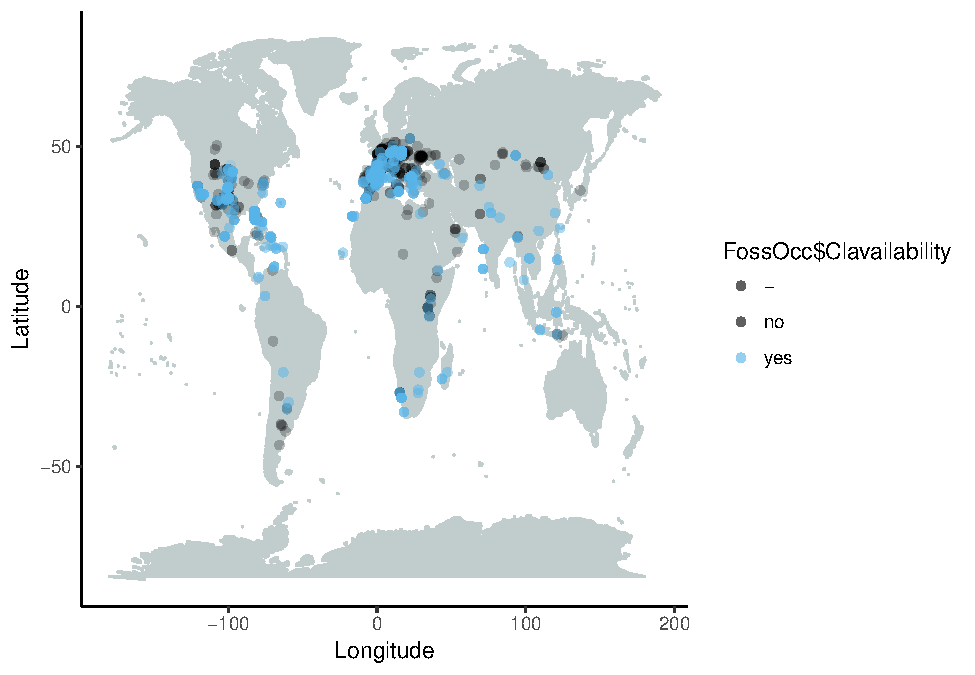
\includegraphics{MA_JJ_files/figure-latex/Map fossil occurrences-1.pdf}
\caption{Map displaying all fossil occurrences of testudinids, with
color indicating whether relevant literature was available (black if
not) and if it was, whether body size data was available or not (yes and
no, respectively).}
\end{figure}

\begin{figure}[htbp]
\centering
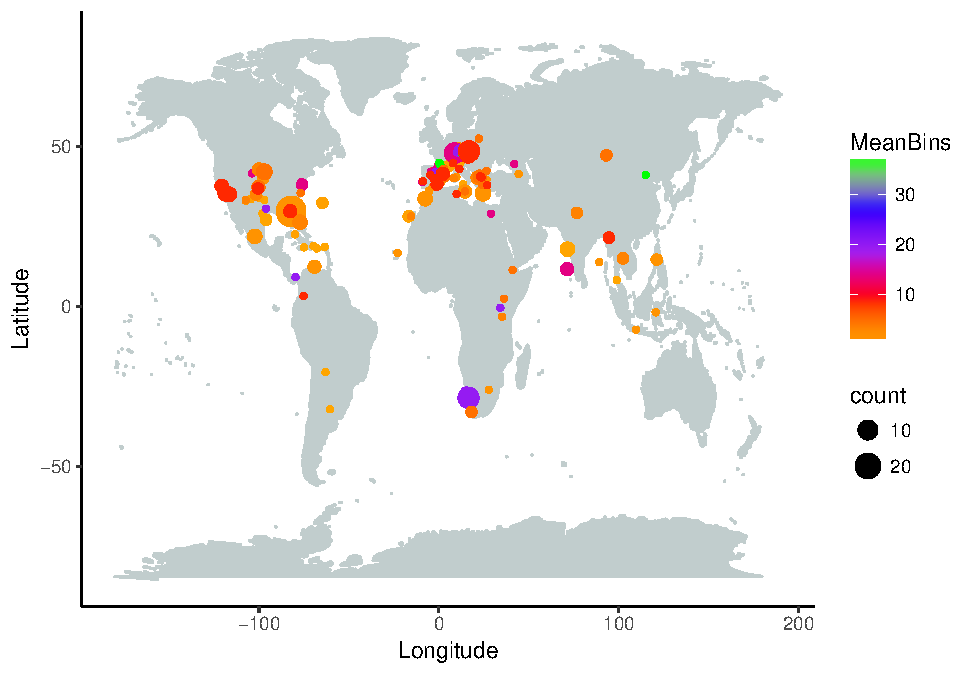
\includegraphics{MA_JJ_files/figure-latex/Map body size data set-1.pdf}
\caption{Map displaying all localities for which body size data for
testudinids was available in the literature. Size of points denotes
sample size, color denotes approximate age.}
\end{figure}

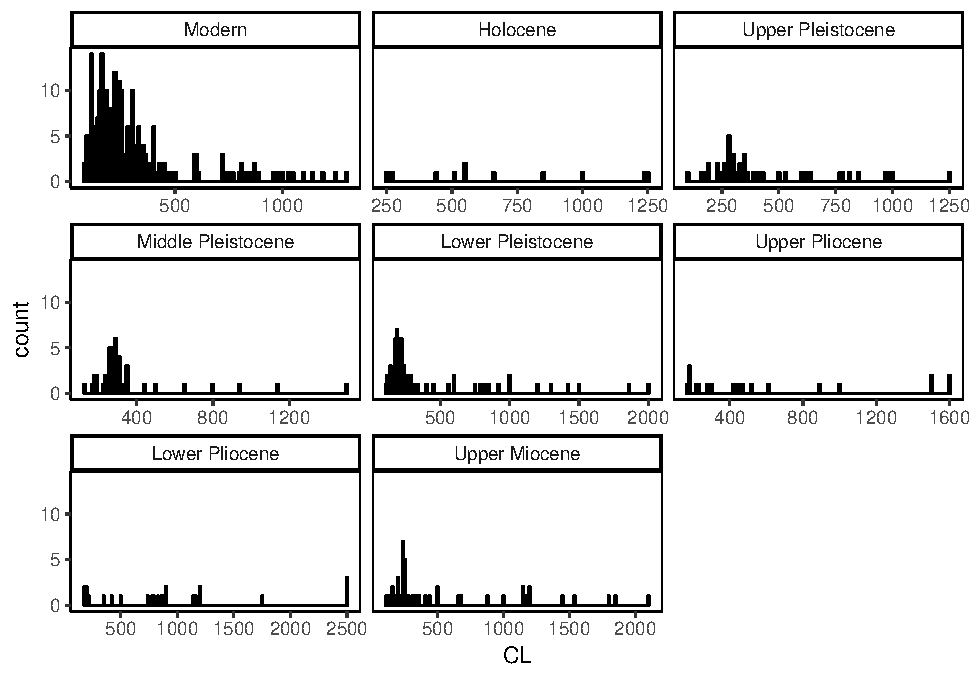
\includegraphics{MA_JJ_files/figure-latex/Histograms of body size data-1.pdf}
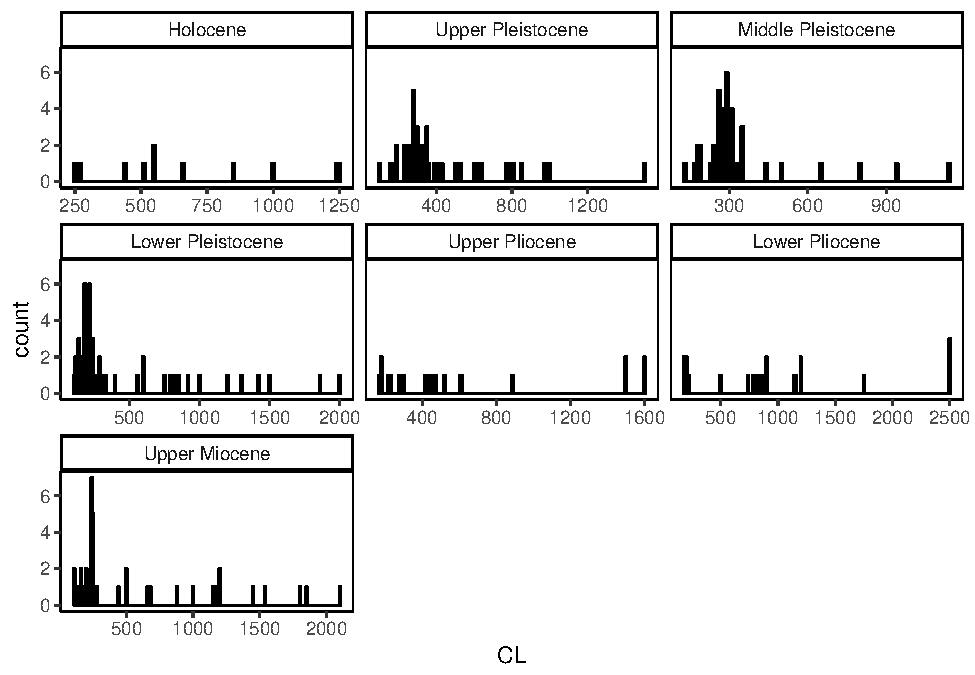
\includegraphics{MA_JJ_files/figure-latex/Histograms of body size data-2.pdf}

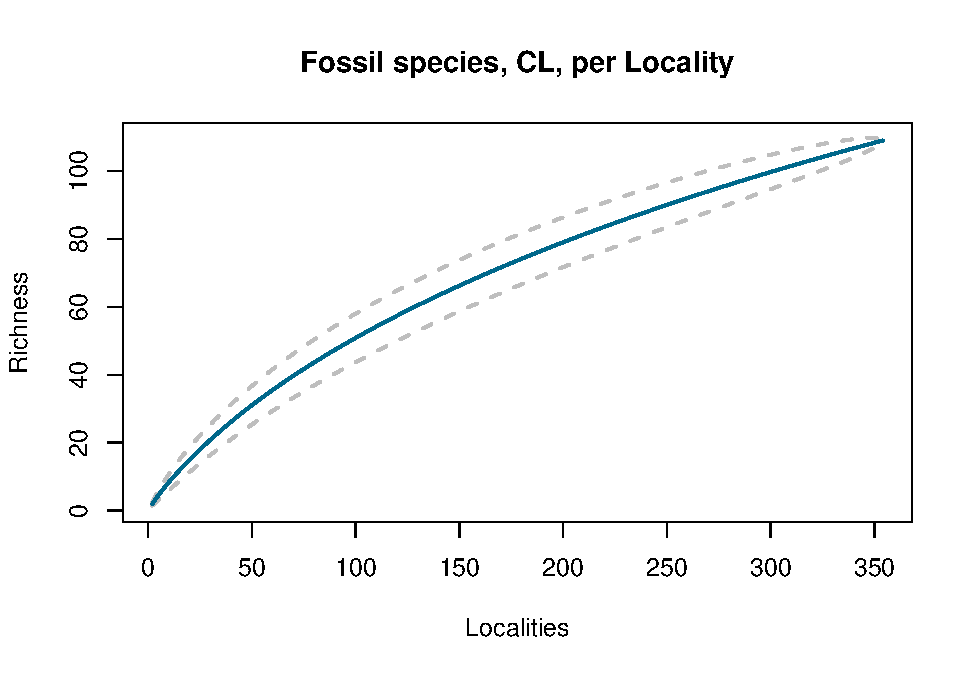
\includegraphics{MA_JJ_files/figure-latex/Species Accumulation Curve-1.pdf}
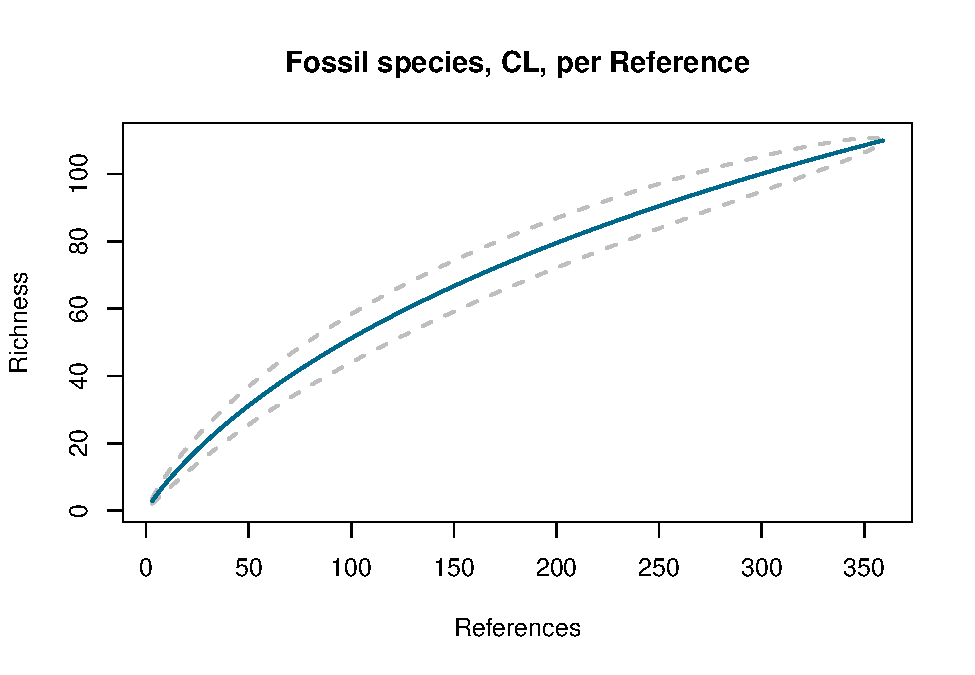
\includegraphics{MA_JJ_files/figure-latex/Species Accumulation Curve-2.pdf}

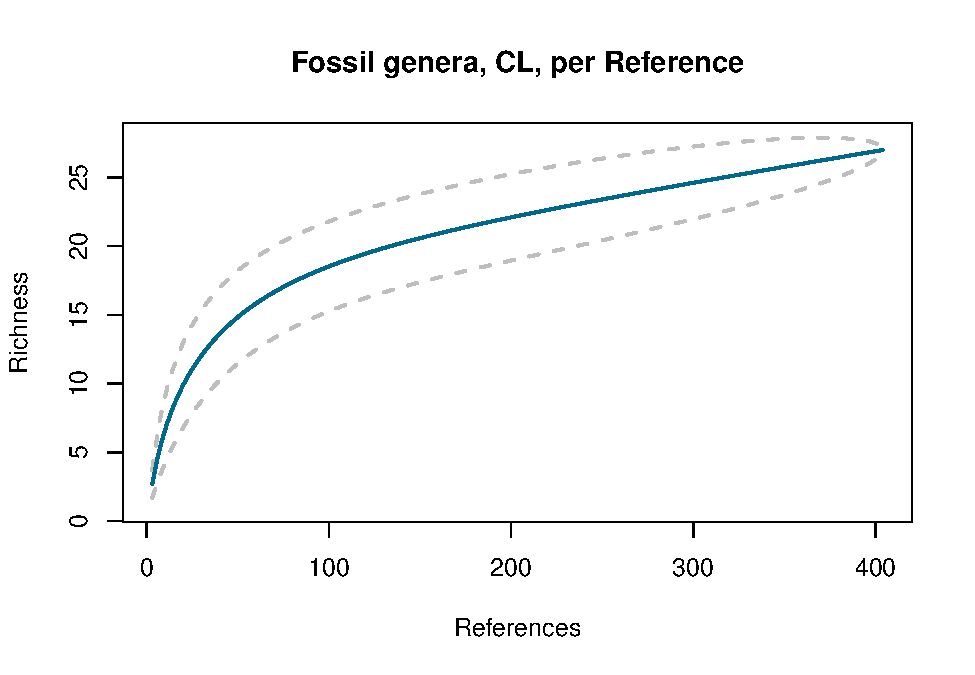
\includegraphics{MA_JJ_files/figure-latex/Species Accumulation Curve with Genera-1.pdf}
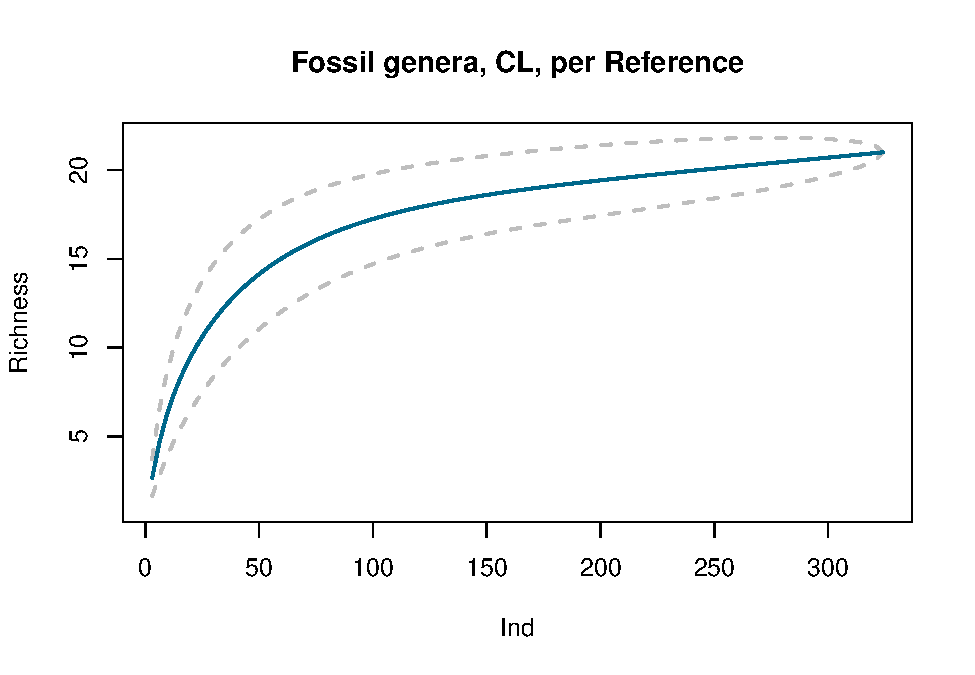
\includegraphics{MA_JJ_files/figure-latex/Species Accumulation Curve with Genera-2.pdf}

\begin{verbatim}
## Warning: Removed 16 rows containing missing values (geom_pointrange).
\end{verbatim}

\begin{figure}[htbp]
\centering
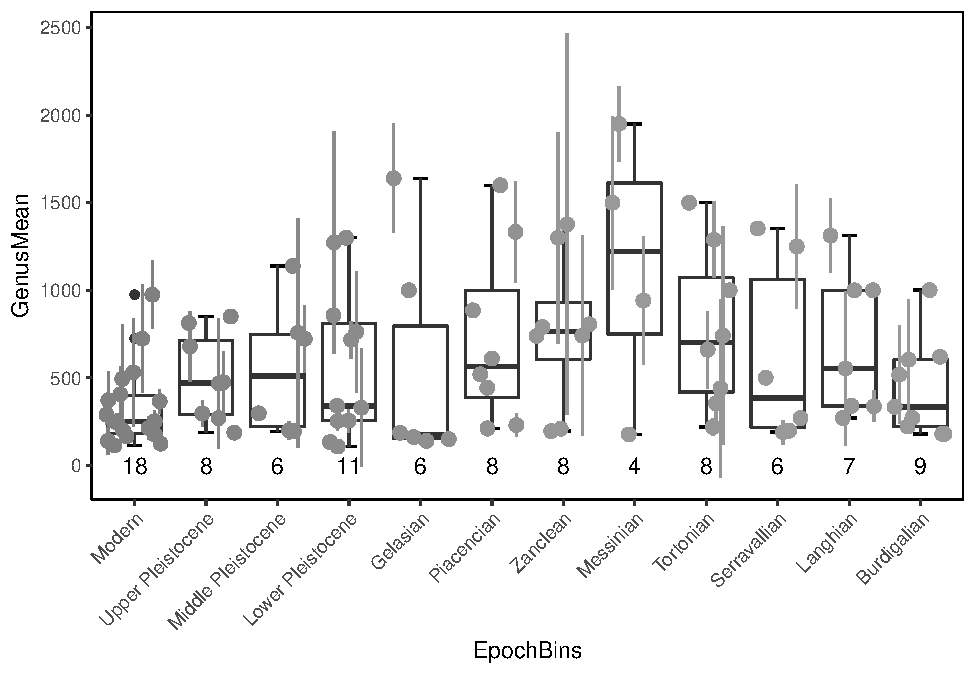
\includegraphics{MA_JJ_files/figure-latex/Boxplots of each genus per time bin-1.pdf}
\caption{Boxplots of each genus per time bin}
\end{figure}

\begin{verbatim}
## Warning: Removed 16 rows containing missing values (geom_pointrange).
\end{verbatim}

\begin{figure}[htbp]
\centering
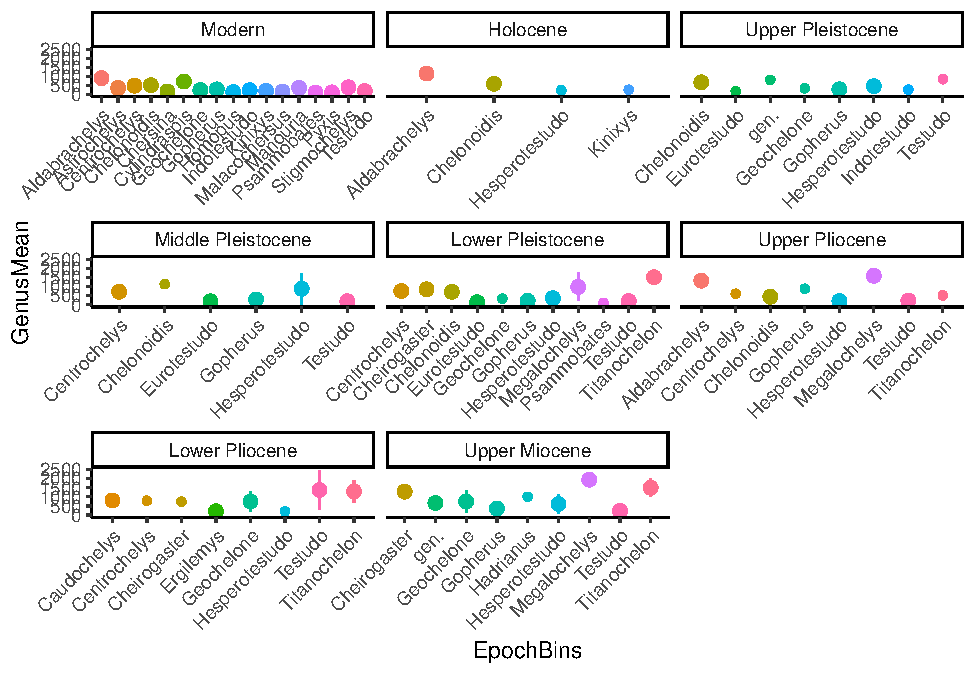
\includegraphics{MA_JJ_files/figure-latex/Separate genera per time bin-1.pdf}
\caption{Mean body size and standard deviation per genus in each time
bin}
\end{figure}

\newpage

\section{including Island species
(n=2215)}\label{including-island-species-n2215}

\begin{longtable}[]{@{}rrrr@{}}
\caption{paleoTS object (mm= mean CL, nn = sample size, vv = variance
(CL), tt = Age)}\tabularnewline
\toprule
mm & nn & vv & tt\tabularnewline
\midrule
\endfirsthead
\toprule
mm & nn & vv & tt\tabularnewline
\midrule
\endhead
246.8335 & 1968 & 2.126636e+09 & 0.0000005\tabularnewline
688.5455 & 11 & 1.245041e+05 & 0.0058500\tabularnewline
447.6480 & 45 & 8.098707e+04 & 0.0688500\tabularnewline
333.8707 & 45 & 3.704545e+04 & 0.4535000\tabularnewline
415.0939 & 66 & 1.833202e+05 & 1.6845000\tabularnewline
642.0167 & 18 & 2.812598e+05 & 3.0940000\tabularnewline
1004.9909 & 22 & 5.319102e+05 & 4.4660000\tabularnewline
582.7750 & 40 & 3.097159e+05 & 8.4700000\tabularnewline
\bottomrule
\end{longtable}

\begin{figure}[htbp]
\centering
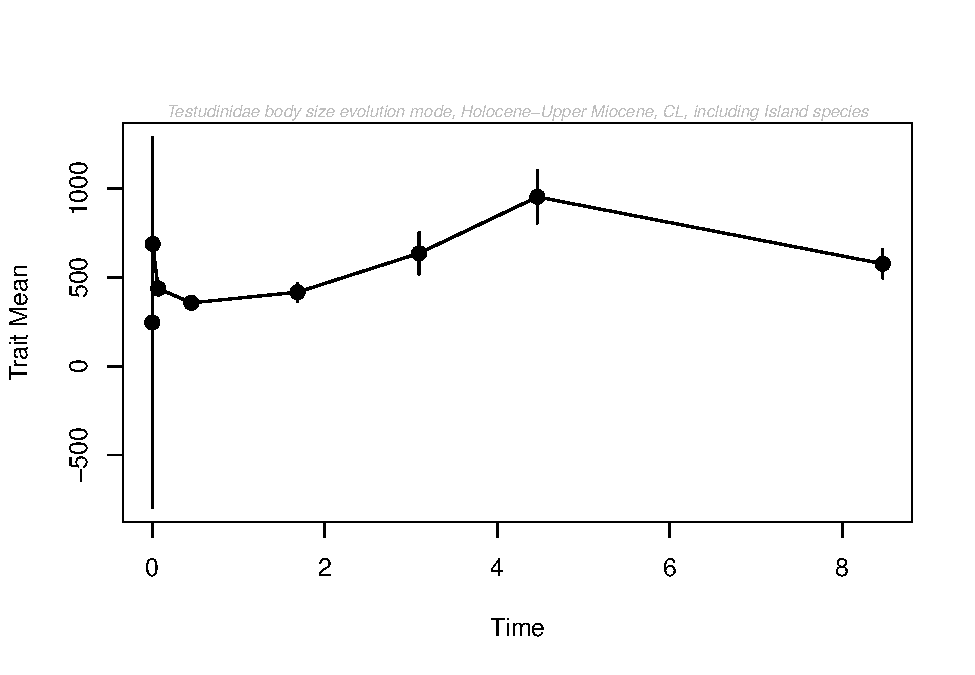
\includegraphics{MA_JJ_files/figure-latex/paleoTS plot-1.pdf}
\caption{individuals, including island species}
\end{figure}

\begin{verbatim}
## 
## Comparing 3 models [n = 7, method = AD]
## 
##             logL K     AICc Akaike.wt
## GRW    -50.30596 2 107.6119     0.038
## URW    -50.78070 1 104.3614     0.191
## Stasis -47.28232 2 101.5646     0.772
\end{verbatim}

\begin{longtable}[]{@{}lrrrr@{}}
\caption{Model-fitting results for testudinidae, individuals, including
island species}\tabularnewline
\toprule
& logL & K & AICc & Akaike.wt\tabularnewline
\midrule
\endfirsthead
\toprule
& logL & K & AICc & Akaike.wt\tabularnewline
\midrule
\endhead
GRW & -50.30596 & 2 & 107.6119 & 0.038\tabularnewline
URW & -50.78070 & 1 & 104.3614 & 0.191\tabularnewline
Stasis & -47.28232 & 2 & 101.5646 & 0.772\tabularnewline
\bottomrule
\end{longtable}

\begin{longtable}[]{@{}lrrr@{}}
\toprule
EpochBins & meanSpeciesCL & nSpecies & MeanBins\tabularnewline
\midrule
\endhead
Holocene & 671.4667 & 5 & 0.00585\tabularnewline
Upper Pleistocene & 521.4533 & 17 & 0.06885\tabularnewline
Middle Pleistocene & 384.8626 & 10 & 0.45350\tabularnewline
Lower Pleistocene & 581.2039 & 28 & 1.68450\tabularnewline
Upper Pliocene & 610.4591 & 11 & 3.09400\tabularnewline
Lower Pliocene & 1009.4738 & 14 & 4.46600\tabularnewline
Upper Miocene & 680.7708 & 24 & 8.47000\tabularnewline
\bottomrule
\end{longtable}

\begin{figure}[htbp]
\centering
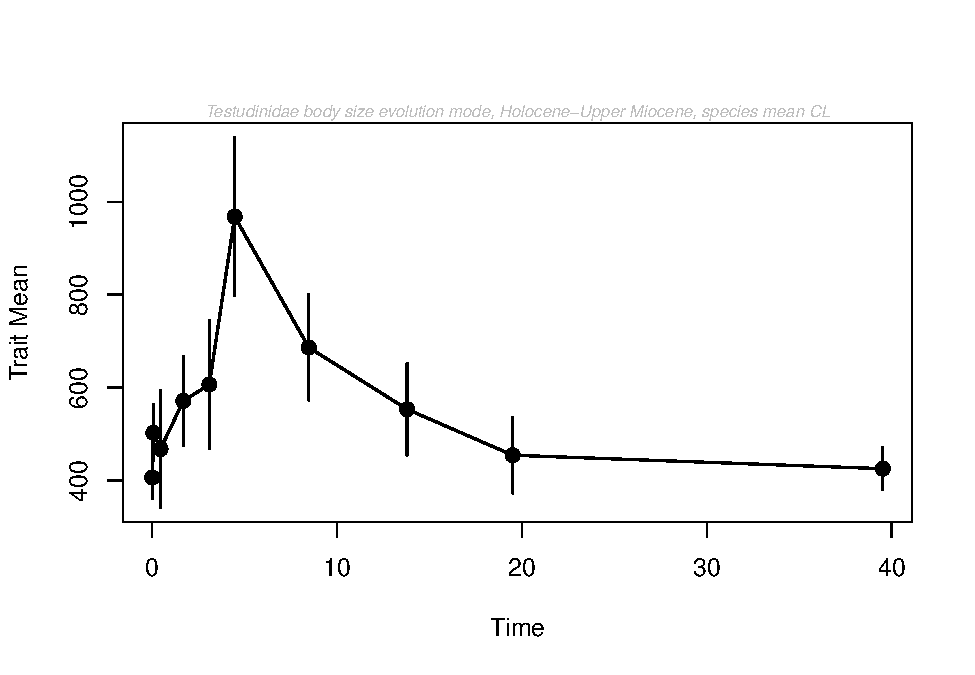
\includegraphics{MA_JJ_files/figure-latex/paleoTS plot with species mean, including island species-1.pdf}
\caption{paleoTS plot with species mean, including island species}
\end{figure}

\begin{longtable}[]{@{}rrrr@{}}
\toprule
tt & mm & vv & nn\tabularnewline
\midrule
\endhead
0.0000005 & 400.5972 & 104321.19 & 50\tabularnewline
0.0058500 & 671.4667 & 195810.92 & 5\tabularnewline
0.0688500 & 521.4533 & 67149.55 & 17\tabularnewline
0.4535000 & 384.8626 & 99603.12 & 10\tabularnewline
1.6845000 & 581.2039 & 319998.46 & 28\tabularnewline
3.0940000 & 610.4591 & 260640.34 & 11\tabularnewline
4.4660000 & 1009.4738 & 437400.60 & 14\tabularnewline
8.4700000 & 680.7708 & 349806.99 & 24\tabularnewline
\bottomrule
\end{longtable}

\begin{figure}[htbp]
\centering
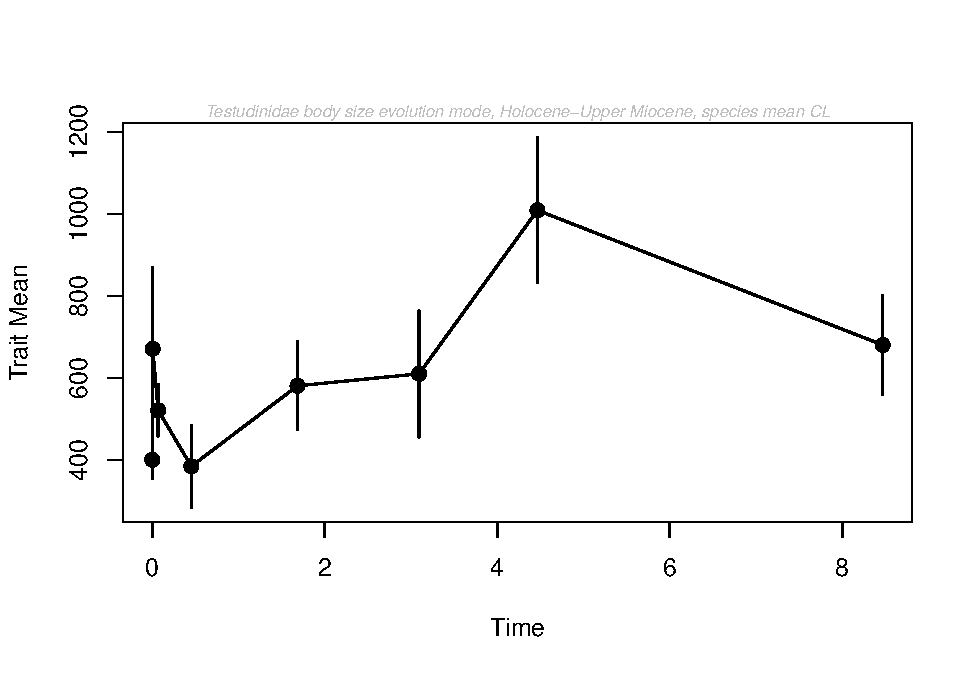
\includegraphics{MA_JJ_files/figure-latex/paleoTS plot with species mean, including island species-2.pdf}
\caption{paleoTS plot with species mean, including island species}
\end{figure}

\begin{verbatim}
## 
## Comparing 3 models [n = 7, method = AD]
## 
##             logL K      AICc Akaike.wt
## GRW    -47.86862 2 102.73724     0.059
## URW    -47.99319 1  98.78638     0.422
## Stasis -45.68754 2  98.37508     0.519
\end{verbatim}

\begin{longtable}[]{@{}lrrrr@{}}
\toprule
& logL & K & AICc & Akaike.wt\tabularnewline
\midrule
\endhead
GRW & -47.86862 & 2 & 102.73724 & 0.059\tabularnewline
URW & -47.99319 & 1 & 98.78638 & 0.422\tabularnewline
Stasis & -45.68754 & 2 & 98.37508 & 0.519\tabularnewline
\bottomrule
\end{longtable}


\end{document}
